\section{Gestion de projet}
    Afin d'assurer le suivi des tâches du projet, le service git gratuit de Microsoft (\url{https://github.com/AgatheLB/leaf_classification_IFT712}) a été utilisé. Il permet non seulement d'utiliser le logiciel de contrôle de versions Git, mais également de créer un tableau de type trello tel que présenté à la figure \ref{fig:trello_board_models}. La méthode kanban dans sa forme la plus simple a été employée pour assigner et suivre les tâches de développement.

    \begin{figure}[H]
        \centering
        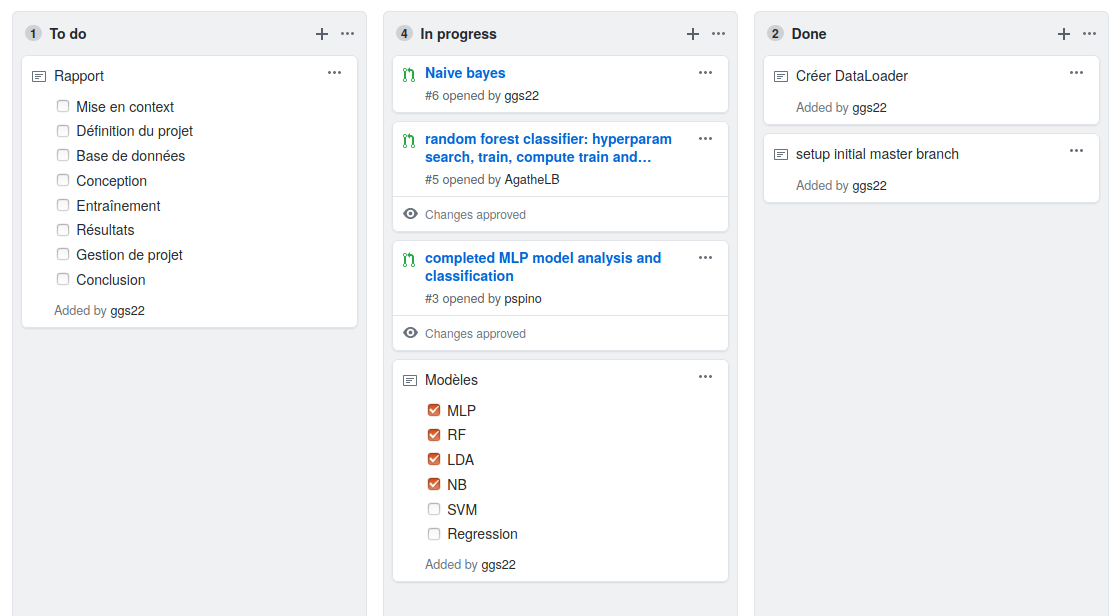
\includegraphics[width=15cm]{images/board.png}
        \caption[Tableau Trello du volet modèles]{Tableau Trello du projet Classifieur de feuilles végétales}
        \label{fig:trello_board_models}
    \end{figure}

    Chaque tâche de développement avait une branche dédiée. Lorsque la tâche était complétée, une \textit{pull request} était créée via l'interface web. Chaque \textit{pull request} a fait l'objet d'une révision par au moins un autre membre de l'équipe. Une fois approuvée et fusionnée, la branche était supprimée.

    Tel que dicté par les bonnes pratiques, il était convenu d'éviter les \textit{commits} introduisant trop de changements. Cela afin de simplifier la tâche de révision, et bien cerner le \textit{scope} des tâches. Il a également été décidé de conserver l'historique entier pour chaque \textit{merge}. La figure \ref{fig:git_graph} montre un aperçu de l'arborescence Git du projet.

    \begin{figure}[H]
        \centering
        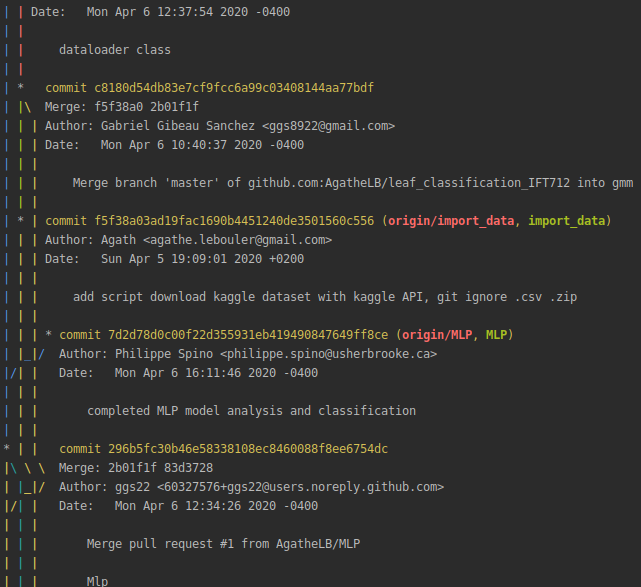
\includegraphics[width=12cm]{images/git_graph.png}
        \caption{Apperçu de l'arborescence du Git}
        \label{fig:git_graph}
    \end{figure}
